%%%%%%%%%%%%%%%%%%%%%%%%%%%%%%%%%%%%%%%%%
% Beamer Presentation
% LaTeX Template
% Version 1.0 (10/11/12)
%
% This template has been downloaded from:
% http://www.LaTeXTemplates.com
%
% License:
% CC BY-NC-SA 3.0 (http://creativecommons.org/licenses/by-nc-sa/3.0/)
%
%%%%%%%%%%%%%%%%%%%%%%%%%%%%%%%%%%%%%%%%%

%----------------------------------------------------------------------------------------
%	PACKAGES AND THEMES
%----------------------------------------------------------------------------------------

\documentclass{beamer}

\mode<presentation> {

% The Beamer class comes with a number of default slide themes
% which change the colors and layouts of slides. Below this is a list
% of all the themes, uncomment each in turn to see what they look like.

%\usetheme{default}
%\usetheme{AnnArbor}
%\usetheme{Antibes}
%\usetheme{Bergen}
%\usetheme{Berkeley}
%\usetheme{Berlin}
%\usetheme{Boadilla}
%\usetheme{CambridgeUS}
%\usetheme{Copenhagen}
%\usetheme{Darmstadt}
%\usetheme{Dresden}
%\usetheme{Frankfurt}
%\usetheme{Goettingen}
%\usetheme{Hannover}
%\usetheme{Ilmenau}
%\usetheme{JuanLesPins}
%\usetheme{Luebeck}
%\usetheme{Madrid}
%\usetheme{Malmoe}
%\usetheme{Marburg}
%\usetheme{Montpellier}
\usetheme{PaloAlto}
%\usetheme{Pittsburgh}
%\usetheme{Rochester}
%\usetheme{Singapore}
%\usetheme{Szeged}
%\usetheme{Warsaw}

% As well as themes, the Beamer class has a number of color themes
% for any slide theme. Uncomment each of these in turn to see how it
% changes the colors of your current slide theme.

%\usecolortheme{albatross}
%\usecolortheme{beaver}
%\usecolortheme{beetle}
%\usecolortheme{crane}
%\usecolortheme{dolphin}
%\usecolortheme{dove}
%\usecolortheme{fly}
%\usecolortheme{lily}
%\usecolortheme{orchid}
%\usecolortheme{rose}
%\usecolortheme{seagull}
%\usecolortheme{seahorse}
%\usecolortheme{whale}
%\usecolortheme{wolverine}

%\setbeamertemplate{footline} % To remove the footer line in all slides uncomment this line
%\setbeamertemplate{footline}[page number] % To replace the footer line in all slides with a simple slide count uncomment this line

%\setbeamertemplate{navigation symbols}{} % To remove the navigation symbols from the bottom of all slides uncomment this line
}

\usepackage{graphicx} % Allows including images
\usepackage{booktabs} % Allows the use of \toprule, \midrule and \bottomrule in tables
\usepackage{multimedia}
\usepackage{hyperref}



%----------------------------------------------------------------------------------------
%	TITLE PAGE
%----------------------------------------------------------------------------------------

\title[FlappyPi]{The Summer C Project and FlappyPi} % The short title appears at the bottom of every slide, the full title is only on the title page

\author[Group 16]{\small Henryk~Haddass \and Mickey~Li \and Michael~Radigan \and Oliver~Wheeler}% Your name
\institute[Imperial DoC] % Your institution as it will appear on the bottom of every slide, may be shorthand to save space
{
Group 16
\medskip
}
\date{\today} % Date, can be changed to a custom date

\begin{document}

\begin{frame}
\titlepage % Print the title page as the first slide
\end{frame}

\begin{frame}
\frametitle{Overview} % Table of contents slide, comment this block out to remove it
\tableofcontents % Throughout your presentation, if you choose to use \section{} and \subsection{} commands, these will automatically be printed on this slide as an overview of your presentation
\end{frame}

%----------------------------------------------------------------------------------------
%	PRESENTATION SLIDES
%----------------------------------------------------------------------------------------

%------------------------------------------------
\section{Emulator} % Sections can be created in order to organize your presentation into discrete blocks, all sections and subsections are automatically printed in the table of contents as an overview of the talk

%------------------------------------------------

\subsection{Implementation} % A subsection can be created just before a set of slides with a common theme to further break down your presentation into chunks



\begin{frame}
\frametitle{Our Approach}

\begin{itemize}
\item We based the design on the structure of the CPU
\item This allowed us to split the design into functional sections
\item We emulated specific functionalities of the CPU with corresponding method names
\item The code was written so as not to be repetitive 
\end{itemize}

\end{frame}
%------------------------------------------------
\begin{frame}
\frametitle{Structure}
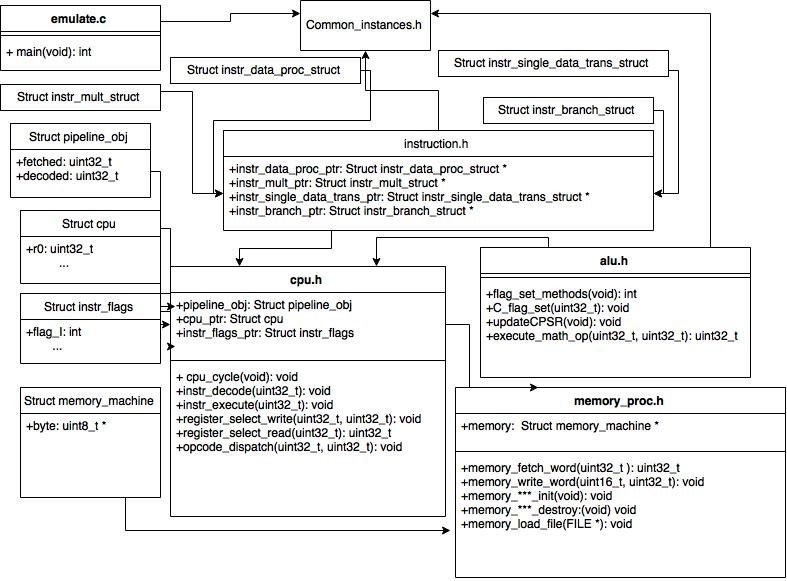
\includegraphics[width=0.9\linewidth]{Images/Emulator_XML(2).jpg}
\end{frame}


%------------------------------------------------
\subsection{Outcome}
\begin{frame}
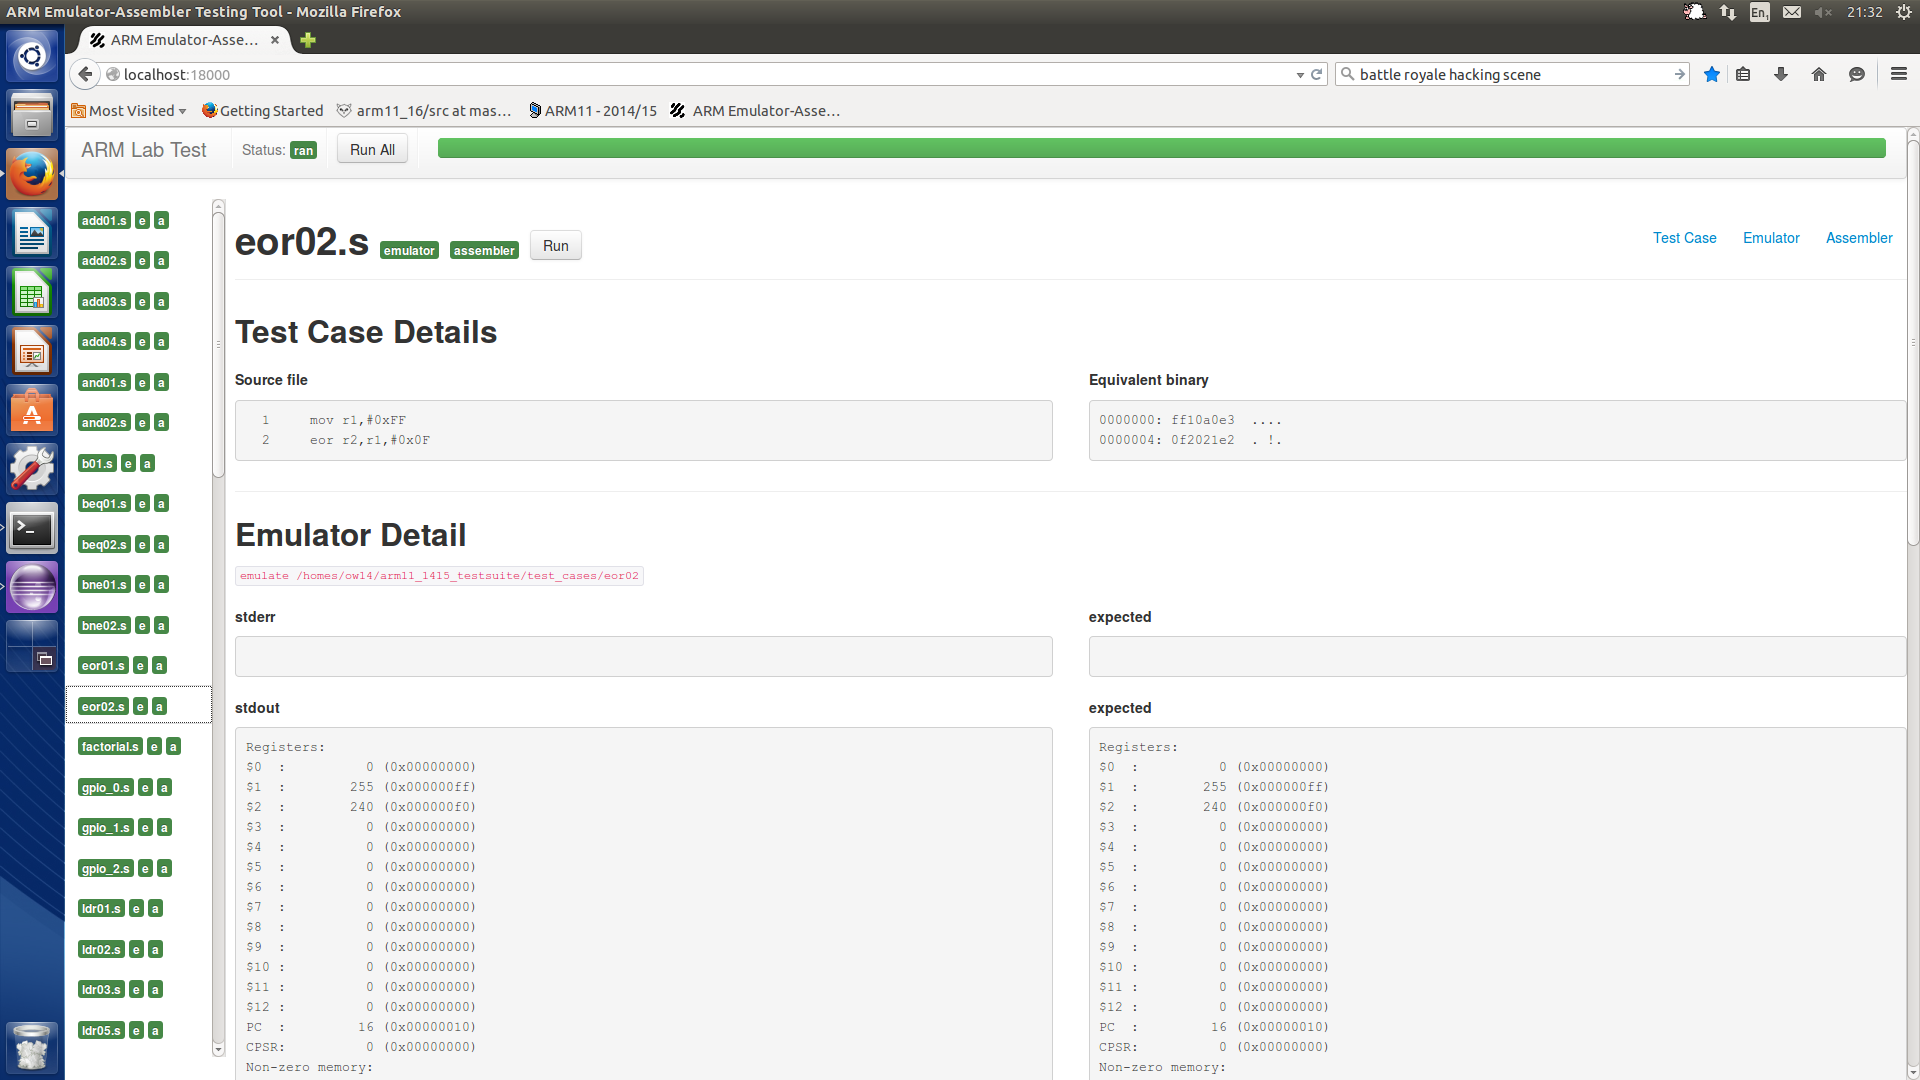
\includegraphics[width=0.9\linewidth]{Images/EmulatorTestCases.png}
\frametitle{Outcome}




\end{frame}

%------------------------------------------------
\subsection{Evaluation}


\begin{frame}
\frametitle{Problems and Challenges}

\begin{description}
\item[Design]\hfill\\
	We were initially unsure of the most efficient (or readable) way to design our implementation.
	
\item[I want to break free]\hfill\\
	We had difficulty freeing pointers in the correct place, leading to segmentation faults
\item[Debugging]\hfill\\
    It took us the same amount of time to debug our code as to write it. We debugged our code by using Eclipse, which was useful in showing us which variable values we had at any given time. Implement a pipeline at the start not at the end, which caused us offset issues   


\end{description}


\end{frame}

%------------------------------------------------

\begin{frame}
\frametitle{Improvements}
\begin{itemize}
\item Make our code more compact and not be as explicit
\item Write our code to be reusable 
\item Plan THEN code
\item A good night's sleep - for general health

\end{itemize}

\end{frame}


%------------------------------------------------
\section{Assembler}
%------------------------------------------------


\subsection{Implementation}

\begin{frame}
\frametitle{Our Approach}

We used a simple 3 modules approach - \textit{assemble.c}, \textit{dictionary.c} and \textit{encode.c}. 
\\~\\

Characteristics of our assembler include: 
\begin{itemize}
\item 2 pass assembler method

\item Polymorphic AVL Tree ADT dictionary

\item Using the Dictionary to map functions to Opcodes

\item Each Function decodes the instruction string themselves

\end{itemize}

\end{frame}

%------------------------------------------------

\begin{frame}
\frametitle{Structure}

\begin{figure}[c]
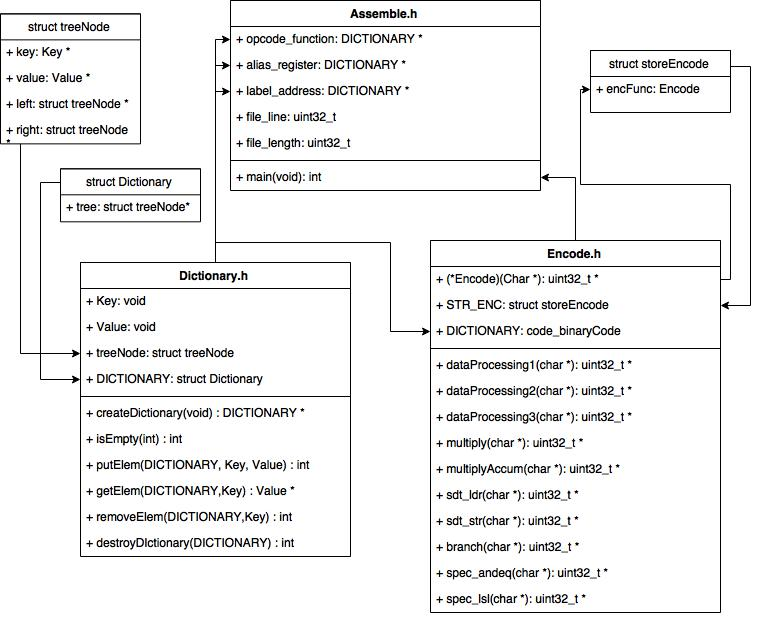
\includegraphics[width=0.9\linewidth]{Images/Assembler_XML.jpg}
\end{figure}


\end{frame}

%------------------------------------------------
\subsection{Outcome}
\begin{frame}[fragile] % Need to use the fragile option when verbatim is used in the slide 
\frametitle{Outcome - Disassembler}

\begin{figure}
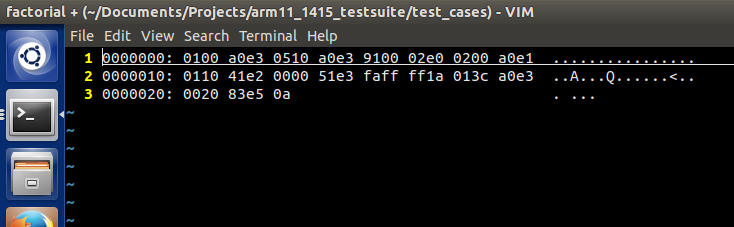
\includegraphics[width=1\linewidth]{Images/Screen1.png}
\end{figure}

\begin{figure}
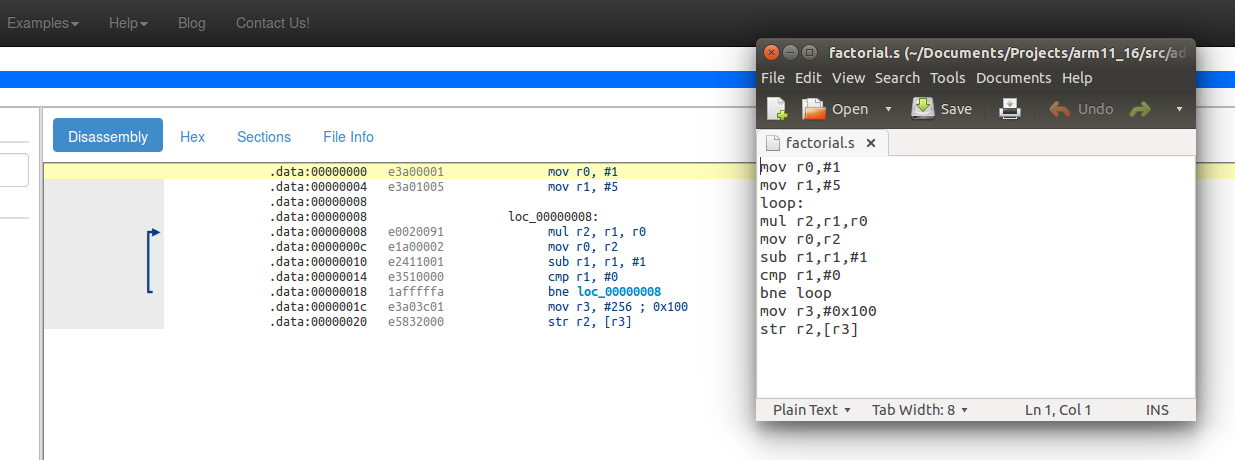
\includegraphics[width=1\linewidth]{Images/Screen2.png}
\end{figure}

\end{frame}

%------------------------------------------------
\subsection{Evaluation}
\begin{frame}
\frametitle{Problems and Challenges}
\begin{description}
\item[String Tokenising]\hfill\\
	Using \textbf{strtok()} and \textbf{sscanf()} proved to be very limiting
	
\item[Dictionary ADT]\hfill\\
	Development of the AVL tree was time consuming and took a long time before it was bug free
	
\item[Memory Allocation]\hfill\\
	Many mistakes and errors ended up being A problem with the use of \textbf{malloc()} and \textbf{free()}.

\item[Code Reuse]\hfill\\
	We definitely could have made a better attempt to reuse code from emulator

\end{description}
\end{frame}

%------------------------------------------------

\begin{frame}
\frametitle{Improvements}
\begin{itemize}
	\item Creating our own string tokeniser which is more flexible then the implementation of \textbf{strtok()}.
	\item Spending a bit more time optimising and improving the quality of the code.
	\item Reducing redundant code
	\item Rethinking the use of pointers
\end{itemize}
\end{frame}

%------------------------------------------------
\section{Proof of use}
%------------------------------------------------
\begin{frame}
\frametitle{Flashing GPIO}

\begin{figure}
\movie[width=3cm,height=2cm,poster]{}{.mp4}
%\movie[width=3cm,height=2cm,poster]{}{test1.mpg}

%\movie[label=cells,width=4cm,height=3cm,poster,showcontrols,duration=5s]{}{test1.mpg}
%\hyperlinkmovie[start=5s,duration=7s]{cells}{\beamerbutton{Show the middle stage}}
%\hyperlinkmovie[start=12s,duration=5s]{cells}{\beamerbutton{Show the late stage}}

\caption{Our Flashing Gpio Led}
\end{figure}


\end{frame}
%------------------------------------------------
\section{Extension}
%------------------------------------------------

\subsection{Implementation}

\begin{frame}
\frametitle{FlappyPi}





\end{frame}

%------------------------------------------------
\begin{frame}
\frametitle{Extending the Assembler}
To make it possible for us to use our own Assembler to process the assemble source code, we have had to do the following:
\begin{description}

\item[Stack (block data transfer)]\hfill\\
	\small Enabling the use of \textbf{stm} and \textbf{ldm} in the assembler, so that the stack can be utilised.
	
\item[Opcodes Suffixes]\hfill\\
	Supporting the addition of condition codes appended to existing opcodes.

\item[Aliasing]\hfill\\
	Supporting the aliasing of registers and commands for clearer use code.
		
\item[Commenting]\hfill\\
	Supporting commenting for clearer programs.

\item[Multi-File Programs]\hfill\\
	Enabling the use of larger programs.

\end{description}
\end{frame}
%------------------------------------------------
\subsection{Outcome}

\begin{frame}
\frametitle{Problems and Challenges - Assembler extension}
\begin{description}
\item[Aliasing]\hfill\\
	Memory corruption due to lack of compatibility with our dictionary
\item[push/pop]\hfill\\
	Difficult to debug as the error was very hard to find
\end{description}
\end{frame}

%------------------------
\begin{frame}
\frametitle{Problems and Challenges - FlappyPi}
\begin{description}
\item[Lack of resources]\hfill\\
There is a small number of helpful articles online covering assembly,
As a result it was difficult to implement.
However, the Cambridge bakingPi tutorial was very helpful for the screen output
\item[Tedious]
Flappy bird sprite was 1200+ lines of assembly which was very repetitive
\end{description}
\end{frame}

%------------------------------------------------
\subsection{Evaluation}

\begin{frame}
\frametitle{Improvements}
\begin{itemize}
\item Stop the bird form flashing
\item Randomly generate terrain
\item Include a button and the ability to move the bird
\item Collision detection to allow the game to be played
\end{itemize}



\end{frame}


%-------------------------------------------------
\section{Project Evaluation}
%-------------------------------------------------
\subsection{Evaluation}
\begin{frame}

\frametitle{Problems and Challenges}

\begin{description}

\item[Organisation]\hfill\\
	\begin{itemize}
	\item Lack of a Complete Plan from the start
	\item Redundant code
	\item Regularly missed personal deadlines
	\item Distribution of tasks
	\end{itemize}

\item[Communication]\hfill\\
	\begin{itemize}
	\item Instant messenger issues
	\item Lack of Clarity
	\item Sleeping Pattens
	\end{itemize}

\item[Effectiveness]\hfill\\
	\begin{itemize}
	\item C knowledge
	\item Testing and Debugging
	\item Git
	\end{itemize}


\end{description}
\end{frame}
%-------------------------------------------------

\begin{frame}
\frametitle{Use of GIT}


\begin{columns}[T] % contents are top vertically aligned
     \begin{column}[T]{4cm} % each column can also be its own environment
     We did not use Git effectively nor efficiently
		\begin{itemize}
			\item Branching
			\item Merging
			\item Excessive use of Master Branch
			\item Non-compiling/ broken code regularly pushed
		\end{itemize}
     \end{column}
     
     \begin{column}[T]{2.5cm} % alternative top-align that's better for graphics
          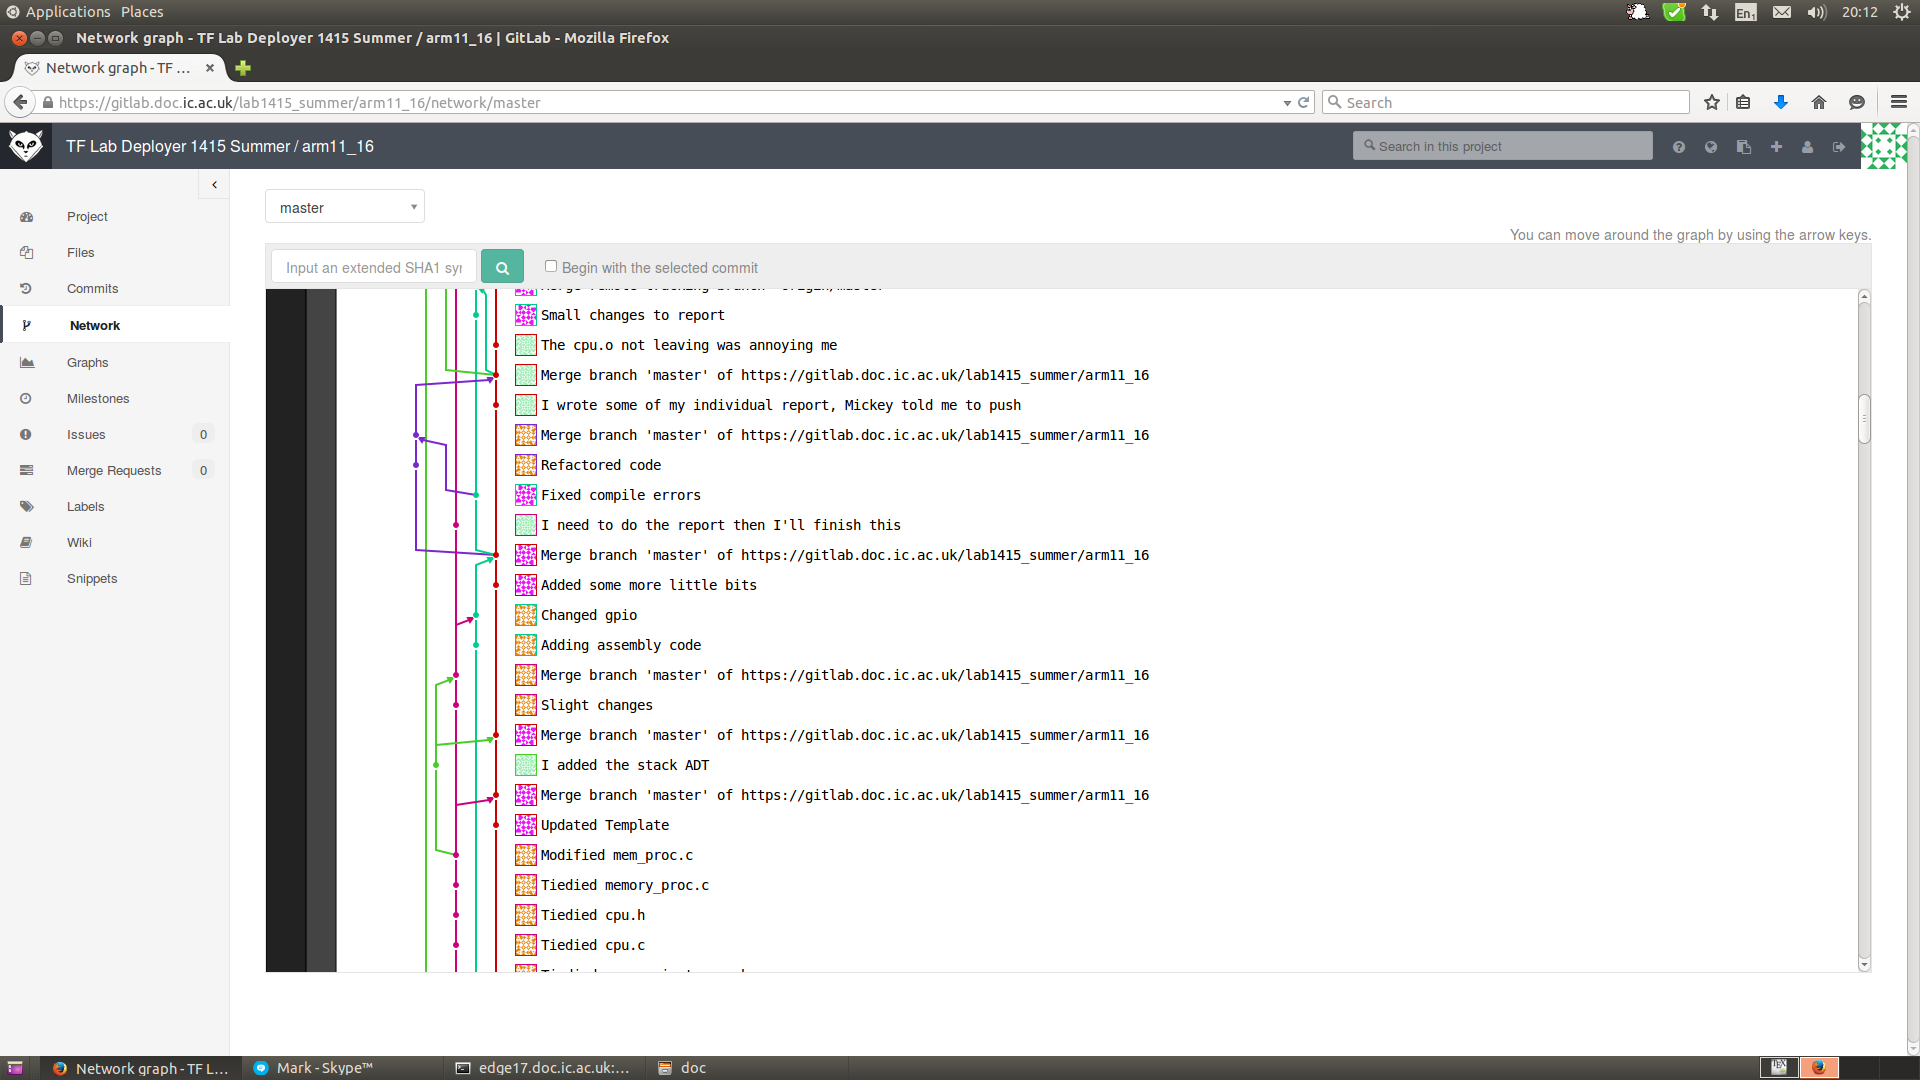
\includegraphics[height=6cm,width=1\linewidth]{Images/Screen3.png}
     \end{column}
     
     \begin{column}[T]{2.5cm} % alternative top-align that's better for graphics
          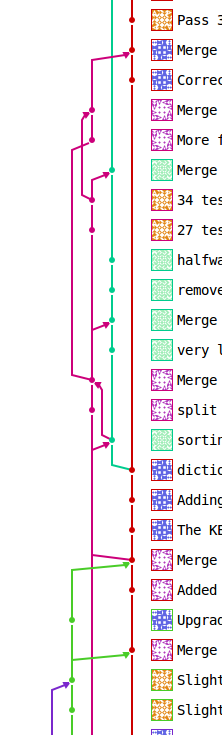
\includegraphics[height=6cm,width=1\linewidth]{Images/Screen4.png}
     \end{column}
     
\end{columns}
\end{frame}


%-------------------------------------------------
\subsection{Improvements}
\begin{frame}

\frametitle{Improvements}





\end{frame}

%-------------------------------------------------
\begin{frame}

\frametitle{Conclusion}





\end{frame}


\end{document} 